\chapter{Perancangan}
\label{chap:perancangan}

\section{Perancangan KIRI \textit{Dashboard Server Side}}
\label{sec:perancangan_kiri_dashboard_server_side}
Seperti yang telah dijelaskan pada bab analisis, bahwa untuk memodelkan KIRI \textit{Dashboard Server Side} dalam Play Framework membutuhkan \textit{models}, \textit{views}, dan \textit{controllers}. Rancangan MVC Play Framework akan dijelaskan pada subbab selanjutnya.

\begin{figure}[htbp]
	\centering
		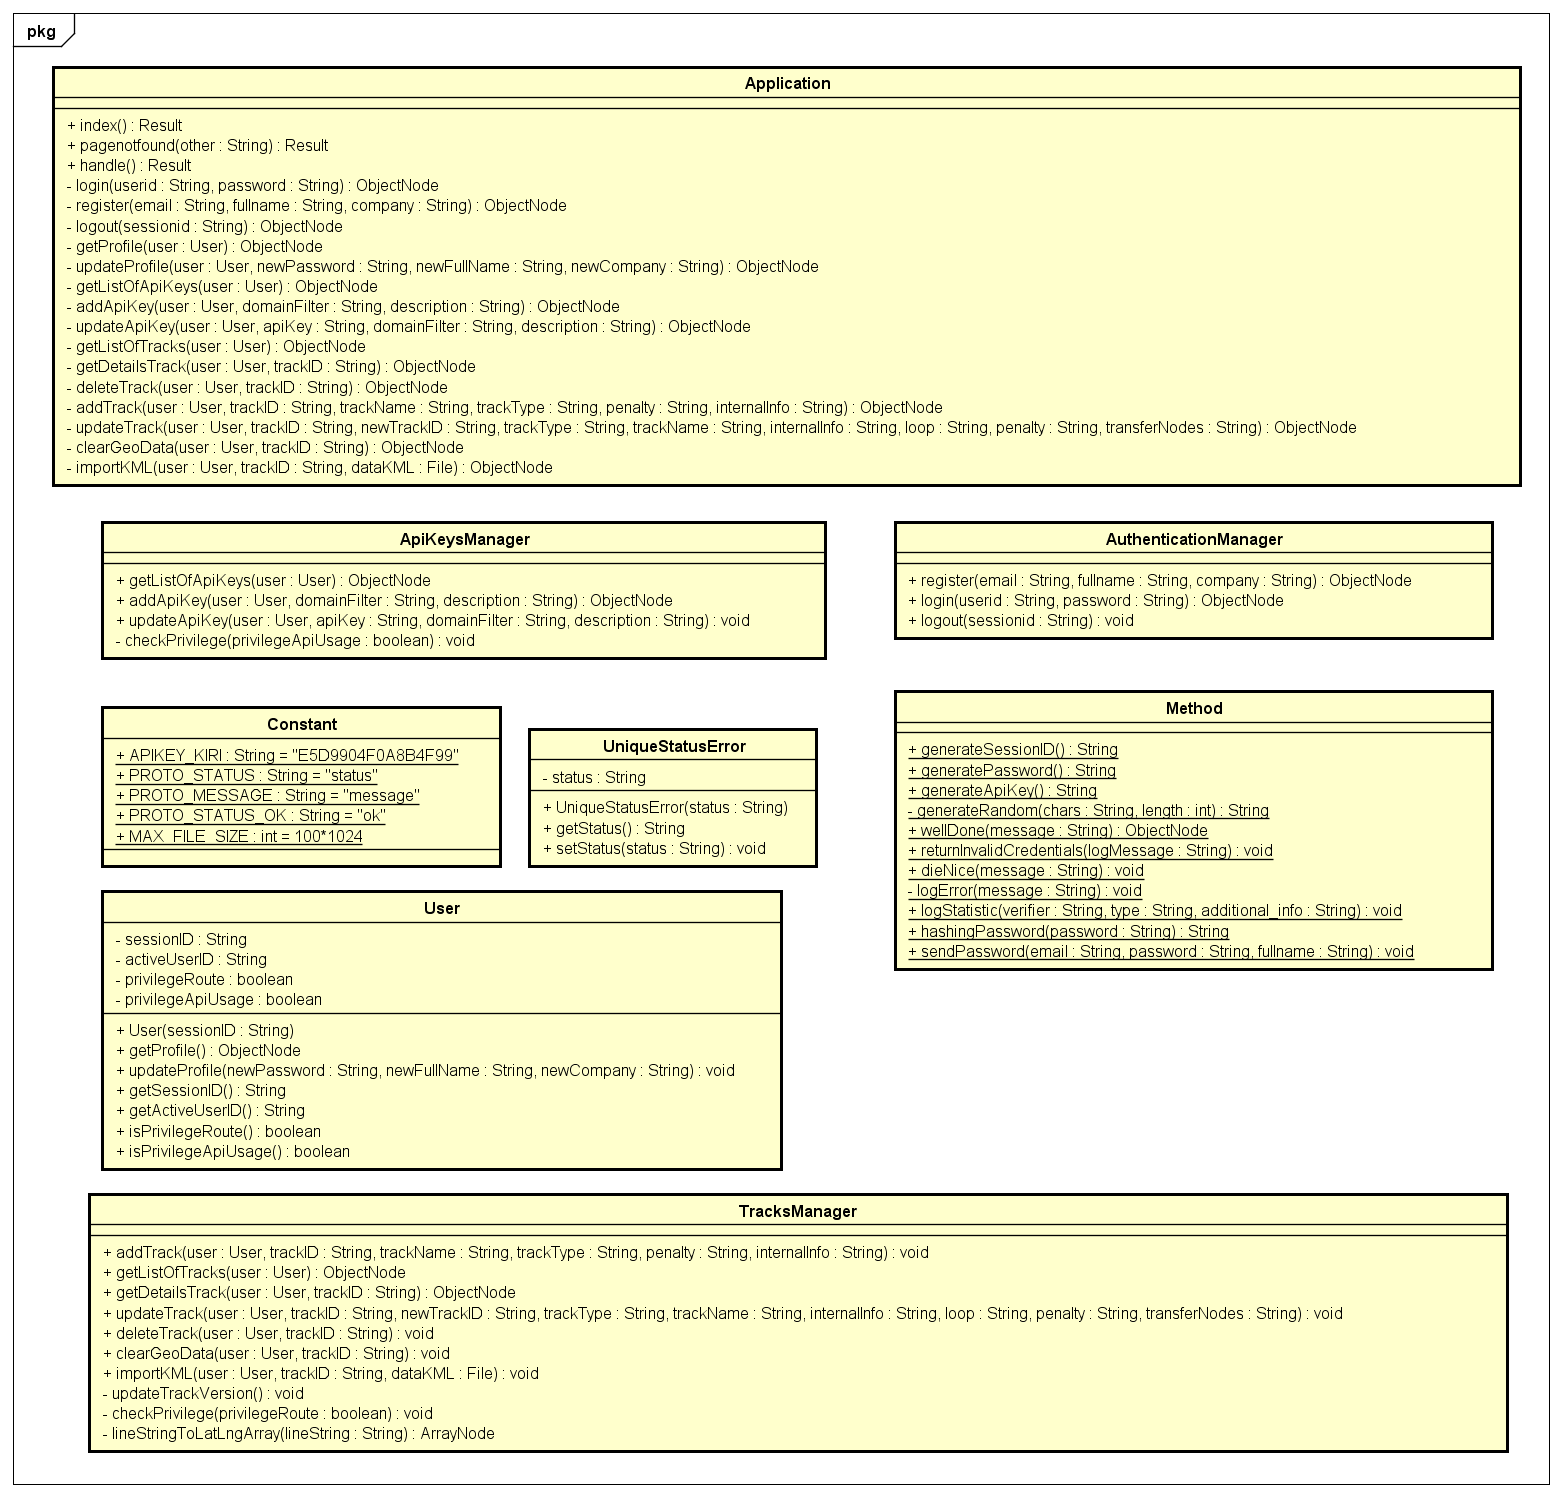
\includegraphics[scale=0.4]{Gambar/4_classdiagram.png}
	\caption{Kelas Diagram KIRI \textit{Dashboard Server Side}}
	\label{fig:4_classdiagram}
\end{figure}

\subsection{\textit{Models}}
\label{sec:modelsrancangan}
\textit{Models} terdiri dari 7 buah kelas. Deskripsi kelas beserta fungsi dari kelas tersebut adalah sebagai berikut:
\begin{enumerate}
	\item ApiKeysManager

	Kelas ini adalah sebagai pengelola \textit{Api Keys} sistem KIRI.
	\item AuthenticationManager

	Kelas ini adalah sebagai pengelola \textit{login}, \textit{logout}, dan \textit{register} pengguna.
	\item Constant

	Kelas ini sebagai pembangun konstanta-konstanta yang bersifat statis.
	\item Method

	Kelas ini sebagai pembangun metode-metode yang digunakan sistem.
	\item TracksManager

	Kelas ini adalah sebagai pengelola rute angkutan umum sistem KIRI.
	\item UniqueStatusErrror

	Kelas ini adalah sebagai pengelola kesalahan sistem.
	\item User

	Kelas ini adalah sebagai pengelola data-data pengguna.
\end{enumerate}

\subsection{\textit{Views}}
\label{sec:viewssrancangan}
Disalin apa adanya.

\subsection{\textit{Controllers}}
\label{sec:controllerssrancangan}
\textit{Controllers} terdiri dari sebuah kelas, yaitu kelas Application. Deskripsi metode-metode beserta fungsi dari kelas Application adalah sebagai berikut:
\begin{itemize}
	\item public Result index()
	\item public Result pagenotfound(String other)
	\item public Result handle()
	\item 16 metode lainnya
\end{itemize}